\documentclass[tikz, border=10pt]{standalone}
\usepackage{tikz}

\usetikzlibrary{arrows, decorations.pathmorphing, decorations.markings, shapes.geometric, calc, positioning}

\tikzset{
    node0/.style={circle, draw, fill=white, inner sep=0pt, minimum size=1.5mm},
    node1/.style={circle, draw, fill=black, inner sep=0pt, minimum size=1.5mm},
    reoEdge/.style={->, >=latex, thin},
    reoSpout/.style={<->, >=latex, thin},
    reoLossy/.style={->, >=latex, thin, dashed},
    reoWavy/.style={->, >=latex, thin, decorate, decoration={zigzag, amplitude=1mm, segment length=1.5mm, post length=1.5mm, pre length=1.5mm}},
}

% A. 基础连线类 (Sync, Lossy, Filter)  参数: #1=样式(可选), #2=起点, #3=终点, #4=标签文字(可选)
\newcommand{\drawLink}[4][reoEdge]{
    \draw[#1] (#2) -- node[above, font=\scriptsize] {#4} (#3);
}

% B. FIFO 类 (中间带方框)  参数: #1=起点, #2=终点, #3=方框内文字, #4=额外样式(可选,如 dashed)
\newcommand{\drawFIFO}[4][]{
    \draw[reoEdge, #1] (#2) -- node[midway, sloped, allow upside down, draw, fill=white, rectangle, minimum width = 6mm, minimum height = 2mm, inner sep=1pt, font=\tiny] {#4} (#3);
}

% C. Drain 类 (两头向中间汇聚)  参数: #1=起点1, #2=起点2, #3=汇聚点/符号位置(通常是这两个点的中点), #4=中心符号(如 ||)
\newcommand{\drawDrain}[5]{
    % 计算中点
    \coordinate (mid1) at ($(#1)!0.4!(#2)$);
    \coordinate (mid) at ($(#1)!0.5!(#2)$);
    \coordinate (mid2) at ($(#1)!0.6!(#2)$);
    % 画两段箭头指向中点
    \draw[->, >=latex, thin] (#1) -- (mid1);
    \draw[thin] (mid1) -- (mid);
    \draw[thin] (mid) -- (mid2);
    \draw[->, >=latex, thin] (#2) -- (mid2);
    % 画中心符号
    \node at (mid) [font=\tiny, inner sep=1pt] {#3};
    \node at (mid1) [font=\tiny, inner sep=1pt] {#4};
    \node at (mid2) [font=\tiny, inner sep=1pt] {#5};
    % 实际上 Drain 并没有显式的 Sink 节点,这里 #3 只是为了兼容位置逻辑,或者如果不画节点只画线
}

% D. Spout 类 (一点分发给两点)  参数: #1=源点, #2=终点1, #3=终点2, #4=线样式
\newcommand{\drawSpout}[5]{
    % 计算中点
    \coordinate (mid1) at ($(#1)!0.4!(#2)$);
    \coordinate (mid) at ($(#1)!0.5!(#2)$);
    \coordinate (mid2) at ($(#1)!0.6!(#2)$);
    % 画两段箭头指向中点
    \draw[->, >=latex, thin] (mid1) -- (#1);
    \draw[thin] (mid1) -- (mid);
    \draw[thin] (mid) -- (mid2);
    \draw[->, >=latex, thin] (mid2) -- (#2);
    % 画中心符号
    \node at (mid) [font=\tiny, inner sep=1pt] {#3};
    \node at (mid1) [font=\tiny, inner sep=1pt] {#4};
    \node at (mid2) [font=\tiny, inner sep=1pt] {#5};
    % 实际上 Drain 并没有显式的 Sink 节点,这里 #3 只是为了兼容位置逻辑,或者如果不画节点只画线
}

% E. Timer 类 (中间带圆角框)  参数: #1=起点, #2=终点, #3=延迟时间 t
\newcommand{\drawTimer}[3]{
    \draw[reoEdge] (#1) -- node[draw, fill=white, rectangle, rounded corners=2pt, minimum size=3.5mm, inner sep=1pt, font=\tiny] (timerbox) {#3} (#2);
}

% F. 复杂 Timer 类 (带控制端口 OFF/RESET/EXPIRE)  参数: #1=起点, #2=终点, #3=延迟时间 t, #4=控制类型(OFF/RST/EXP), #5=控制节点位置(above/below)
\newcommand{\drawComplexTimer}[5]{
    % 先画基础 Timer
    \draw[reoEdge] (#1) -- node[draw, fill=white, rectangle, rounded corners=2pt, minimum size=3.5mm, inner sep=1pt, font=\tiny] (timerbox) {#3} (#2);
    % 画控制端口
    \node (ctrl) [#5=0.5cm of timerbox, font=\tiny] {#4};
    \draw[->, >=latex, dashed] (ctrl) -- (timerbox);
}


% --- 1. Basic Channels ---
\newcommand{\chanSync}[2]{\drawLink{#1}{#2}{}}
\newcommand{\chanLossySync}[2]{\drawLink[reoLossy]{#1}{#2}{}}
\newcommand{\chanSyncDrain}[2]{\drawDrain{#1}{#2}{}{}{}} % 空心汇聚
\newcommand{\chanAsynDrain}[2]{\drawDrain{#1}{#2}{$||$}{}{}} % 带竖线汇聚
% --- 2. FIFO Variants ---
\newcommand{\chanFifoOne}[2]{\drawFIFO{#1}{#2}{}}          % Buffer size 1
\newcommand{\chanFifoN}[3]{\drawFIFO{#1}{#2}{$N=#3$}}      % Buffer size n
\newcommand{\chanFifoOneE}[3]{\drawFIFO{#1}{#2}{$#3$}}     % Initialized with e
\newcommand{\chanFifoNE}[4]{\drawFIFO{#1}{#2}{$#3$}}    % Initialized e with size n
% --- 3. Filter & Producer ---
\newcommand{\chanFilterP}[3]{\drawLink[reoWavy]{#1}{#2}{$P(#3)$}} 
\newcommand{\chanProducerP}[3]{\drawLink{#1}{#2}{Prod: $#3$}} 
% --- 4. Spouts ---
\newcommand{\chanSyncSpout}[2]{\drawSpout{#1}{#2}{}{}{}}
\newcommand{\chanAsynSpout}[2]{\drawSpout{#1}{#2}{$||$}{}{}}
% --- 5. Probabilistic/Faulty ---
\newcommand{\chanCptSync}[3]{\drawLink{#1}{#2}{$p=#3$}}       % Corrupting Sync
\newcommand{\chanRdmSync}[3]{\drawLink{#1}{#2}{#3}}         % Random Sync
\newcommand{\chanProbLossy}[3]{\drawLink[reoLossy]{#1}{#2}{$p=#3$}} % Probabilistic Lossy
\newcommand{\chanFtyFifoOne}[3]{\drawFIFO{#1}{#2}{Fty:$#3$}} % Faulty FIFO
\newcommand{\chanLossyFifoOne}[3]{\drawFIFO[dashed]{#1}{#2}{Lossy:$#3$}} % Lossy FIFO
% --- 6. Timers ---
\newcommand{\chanTimert}[3]{\drawTimer{#1}{#2}{#3}}
\newcommand{\chanOFFTimert}[3]{\drawComplexTimer{#1}{#2}{#3}{OFF}{above}}
\newcommand{\chanRSTTimert}[3]{\drawComplexTimer{#1}{#2}{#3}{RST}{above}}
\newcommand{\chanEXPTimert}[3]{\drawComplexTimer{#1}{#2}{#3}{EXP}{above}}

\begin{document}

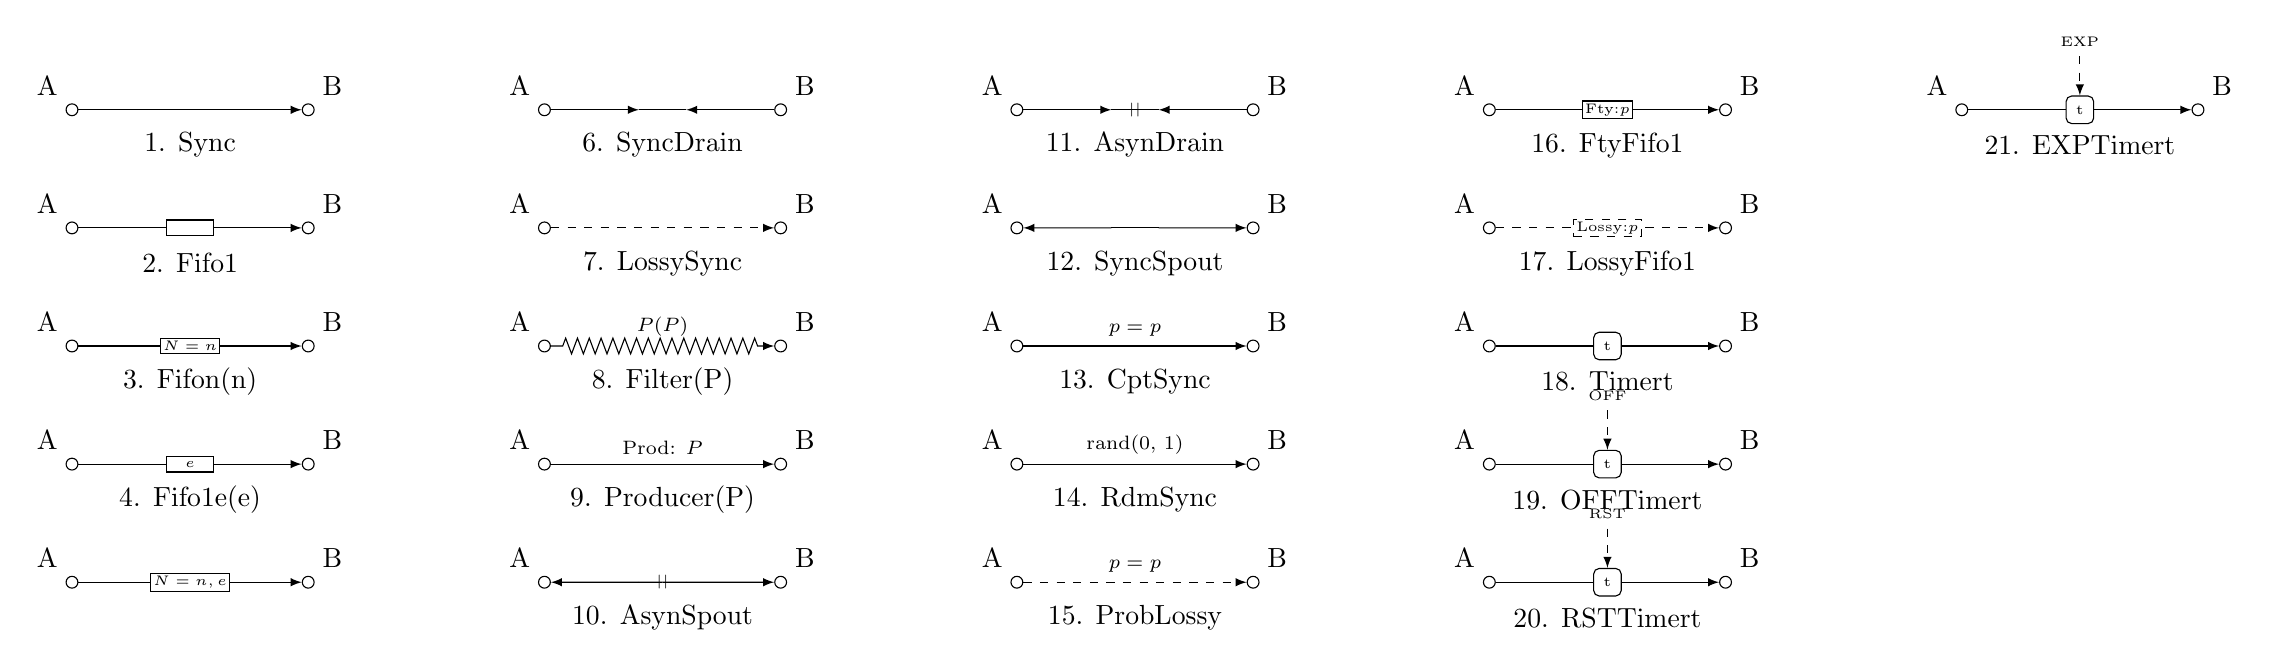
\begin{tikzpicture}[x=3cm, y=1.5cm]
    
    % 1. Sync
    \node[node0, label=above left:A] (A1) at (0,0) {}; \node[node0, label=above right:B] (B1) at (1,0) {};
    \chanSync{A1}{B1}
    \node at (0.5, -0.3) {1. Sync};

    % 2. Fifo1
    \node[node0, label=above left:A] (A2) at (0,-1) {}; \node[node0, label=above right:B] (B2) at (1,-1) {};
    \chanFifoOne{A2}{B2}
    \node at (0.5, -1.3) {2. Fifo1};

    % 3. Fifon
    \node[node0, label=above left:A] (A3) at (0,-2) {}; \node[node0, label=above right:B] (B3) at (1,-2) {};
    \chanFifoN{A3}{B3}{n}
    \node at (0.5, -2.3) {3. Fifon(n)};

    % 4. Fifo1e
    \node[node0, label=above left:A] (A4) at (0,-3) {}; \node[node0, label=above right:B] (B4) at (1,-3) {};
    \chanFifoOneE{A4}{B4}{e}
    \node at (0.5, -3.3) {4. Fifo1e(e)};

    % 5. Fifone
    \node[node0, label=above left:A] (A5) at (0,-4) {}; \node[node0, label=above right:B] (B5) at (1,-4) {};
    \chanFifoNE{A5}{B5}{N = n, e}
    \node at (0.5, -4.3) {5. Fifone(n, e)};

    % 6. SyncDrain
    \node[node0, label=above left:A] (A6) at (2,0) {}; \node[node0, label=above right:B] (B6) at (3,0) {};
    \chanSyncDrain{A6}{B6}
    \node at (2.5, -0.3) {6. SyncDrain};

    % 7. LossySync
    \node[node0, label=above left:A] (A7) at (2,-1) {}; \node[node0, label=above right:B] (B7) at (3,-1) {};
    \chanLossySync{A7}{B7}
    \node at (2.5, -1.3) {7. LossySync};

    % 8. Filterp
    \node[node0, label=above left:A] (A8) at (2,-2) {}; \node[node0, label=above right:B] (B8) at (3,-2) {};
    \chanFilterP{A8}{B8}{P}
    \node at (2.5, -2.3) {8. Filter(P)};

    % 9. Producerp
    \node[node0, label=above left:A] (A9) at (2,-3) {}; \node[node0, label=above right:B] (B9) at (3,-3) {};
    \chanProducerP{A9}{B9}{P}
    \node at (2.5, -3.3) {9. Producer(P)};

    % 10. AsynSpout
    \node[node0, label=above left:A] (A10) at (2,-4) {}; \node[node0, label=above right:B] (B10) at (3, -4) {};
    \chanAsynSpout{A10}{B10}
    \node at (2.5, -4.3) {10. AsynSpout};

    % 11. AsynDrain
    \node[node0, label=above left:A] (A11) at (4,0) {}; \node[node0, label=above right:B] (B11) at (5,0) {};
    \chanAsynDrain{A11}{B11}
    \node at (4.5, -0.3) {11. AsynDrain};

    % 12. SyncSpout
    \node[node0, label=above left:A] (A12) at (4, -1) {}; \node[node0, label=above right:B] (B12) at (5, -1) {};
    \chanSyncSpout{A12}{B12}
    \node at (4.5, -1.3) {12. SyncSpout};

    % 13. CptSync
    \node[node0, label=above left:A] (A13) at (4,-2) {}; \node[node0, label=above right:B] (B13) at (5,-2) {};
    \chanCptSync{A13}{B13}{p}
    \node at (4.5, -2.3) {13. CptSync};

    % 14. RdmSync
    \node[node0, label=above left:A] (A14) at (4,-3) {}; \node[node0, label=above right:B] (B14) at (5,-3) {};
    \chanRdmSync{A14}{B14}{rand(0, 1)}
    \node at (4.5, -3.3) {14. RdmSync};

    % 15. ProbLossy
    \node[node0, label=above left:A] (A15) at (4,-4) {}; \node[node0, label=above right:B] (B15) at (5,-4) {};
    \chanProbLossy{A15}{B15}{p}
    \node at (4.5, -4.3) {15. ProbLossy};

    % 16. FtyFifo1
    \node[node0, label=above left:A] (A16) at (6,0) {}; \node[node0, label=above right:B] (B16) at (7,0) {};
    \chanFtyFifoOne{A16}{B16}{p}
    \node at (6.5, -0.3) {16. FtyFifo1};

    % 17. LossyFifo1
    \node[node0, label=above left:A] (A17) at (6,-1) {}; \node[node0, label=above right:B] (B17) at (7,-1) {};
    \chanLossyFifoOne{A17}{B17}{p}
    \node at (6.5, -1.3) {17. LossyFifo1};

    % 18. Timert
    \node[node0, label=above left:A] (A18) at (6,-2) {}; \node[node0, label=above right:B] (B18) at (7,-2) {};
    \chanTimert{A18}{B18}{t}
    \node at (6.5, -2.3) {18. Timert};

    % 19. OFFTimert
    \node[node0, label=above left:A] (A19) at (6,-3) {}; \node[node0, label=above right:B] (B19) at (7,-3) {};
    \chanOFFTimert{A19}{B19}{t}
    \node at (6.5, -3.3) {19. OFFTimert};

    % 20. RSTTimert
    \node[node0, label=above left:A] (A20) at (6,-4) {}; \node[node0, label=above right:B] (B20) at (7,-4) {};
    \chanRSTTimert{A20}{B20}{t}
    \node at (6.5, -4.3) {20. RSTTimert};

    % 21. EXPTimert
    \node[node0, label=above left:A] (A21) at (8,0) {}; \node[node0, label=above right:B] (B21) at (9,0) {};
    \chanEXPTimert{A21}{B21}{t}
    \node at (8.5, -0.3) {21. EXPTimert};

\end{tikzpicture}

\end{document}